\documentclass[paper=letter,11pt]{scrartcl}

\KOMAoptions{headinclude=true, footinclude=false}
\KOMAoptions{DIV=14, BCOR=5mm}
\KOMAoptions{numbers=noendperiod}
\KOMAoptions{parskip=half}
\addtokomafont{disposition}{\rmfamily}
\addtokomafont{part}{\LARGE}
\addtokomafont{descriptionlabel}{\rmfamily}
%\setkomafont{pageheadfoot}{\normalsize\sffamily}
\setkomafont{pagehead}{\normalsize\rmfamily}
%\setkomafont{publishers}{\normalsize\rmfamily}
\setkomafont{caption}{\normalfont\small}
\setcapindent{0pt}
\deffootnote[1em]{1em}{1em}{\textsuperscript{\thefootnotemark}\ }


\usepackage{amsmath}
\usepackage[varg]{txfonts}
\usepackage[T1]{fontenc}
\usepackage{graphicx}
\usepackage{xcolor}
\usepackage[american]{babel}
% hyperref is needed in many places, so include it here
\usepackage{hyperref}

\usepackage{xspace}
\usepackage{multirow}
\usepackage{float}


\usepackage{braket}
\usepackage{bbm}
\usepackage{relsize}
\usepackage{tcolorbox}

\def\ketY{\ensuremath{\ket {\Psi}}}
\def\iGeV{\ensuremath{\textrm{GeV}^{-1}}}
%\def\mp{\ensuremath{m_{\textrm{proton}}}}
\def\rp{\ensuremath{r_{\textrm{proton}}}}
\def\me{\ensuremath{m_{\textrm{electron}}}}
\def\aG{\ensuremath{\alpha_G}}
\def\rAtom{\ensuremath{r_{\textrm{atom}}}}
\def\rNucl{\ensuremath{r_{\textrm{nucleus}}}}
\def\GN{\ensuremath{\textrm{G}_\textrm{N}}}
\def\ketX{\ensuremath{\ket{\vec{x}}}}
\def\ve{\ensuremath{\vec{\epsilon}}}


\def\ABCDMatrix{\ensuremath{\begin{pmatrix} A &  B  \\ C  & D \end{pmatrix}}}
\def\xyprime{\ensuremath{\begin{pmatrix} x' \\ y' \end{pmatrix}}}
\def\xyprimeT{\ensuremath{\begin{pmatrix} x' &  y' \end{pmatrix}}}
\def\xy{\ensuremath{\begin{pmatrix} x \\ y \end{pmatrix}}}
\def\xyT{\ensuremath{\begin{pmatrix} x & y \end{pmatrix}}}

\def\IMatrix{\ensuremath{\begin{pmatrix} 0 &  1  \\ -1  & 0 \end{pmatrix}}}
\def\IBoostMatrix{\ensuremath{\begin{pmatrix} 0 &  1  \\ 1  & 0 \end{pmatrix}}}
\def\JThree{\ensuremath{\begin{pmatrix}    0 & -i & 0  \\ i & 0  & 0 \\ 0 & 0 & 0 \end{pmatrix}}} 
\def\JTwo{\ensuremath{\begin{bmatrix}    0 & 0 & -i  \\ 0 & 0  & 0 \\ i & 0 & 0 \end{bmatrix}}}
\def\JOne{\ensuremath{\begin{bmatrix}    0 & 0 & 0  \\ 0 & 0  & -i \\ 0 & i & 0 \end{bmatrix}}}
\def\etamn{\ensuremath{\eta_{\mu\nu}}}
\def\Lmn{\ensuremath{\Lambda^\mu_\nu}}
\def\dmn{\ensuremath{\delta^\mu_\nu}}
\def\wmn{\ensuremath{\omega^\mu_\nu}}
\def\be{\begin{equation*}}
\def\ee{\end{equation*}}
\def\bea{\begin{eqnarray*}}
\def\eea{\end{eqnarray*}}
\def\bi{\begin{itemize}}
\def\ei{\end{itemize}}
\def\fmn{\ensuremath{F_{\mu\nu}}}
\def\fMN{\ensuremath{F^{\mu\nu}}}
\def\bc{\begin{center}}
\def\ec{\end{center}}
\def\nus{$\nu$s}

\def\adagger{\ensuremath{a_{p\sigma}^\dagger}}
\def\lineacross{\noindent\rule{\textwidth}{1pt}}

\newcommand{\multiline}[1] {
\begin{tabular} {|l}
#1
\end{tabular}
}

\newcommand{\multilineNoLine}[1] {
\begin{tabular} {l}
#1
\end{tabular}
}



\newcommand{\lineTwo}[2] {
\begin{tabular} {|l}
#1 \\
#2
\end{tabular}
}

\newcommand{\rmt}[1] {
\textrm{#1}
}


%
% Units
%
\def\m{\ensuremath{\rmt{m}}}
\def\GeV{\ensuremath{\rmt{GeV}}}
\def\pt{\ensuremath{p_\rmt{T}}}


\def\parity{\ensuremath{\mathcal{P}}}

\usepackage{cancel}
\usepackage{ mathrsfs }
\def\bigL{\ensuremath{\mathscr{L}}}

\usepackage{ dsfont }



\usepackage{fancyhdr}
\fancyhf{}


\lhead{\Large 33-444} % \hfill Introduction to Particle Physics \hfill Spring 2020}
\chead{\Large Introduction to Particle Physics} % \hfill Spring 2020}
\rhead{\Large Spring 2020} % \hfill Introduction to Particle Physics \hfill Spring 2020}

\begin{document}
\thispagestyle{fancy}

\begin{center}
{\huge \textbf{Lecture 23}}
\end{center}

{\fontsize{14}{16}\selectfont


\fbox{\begin{minipage}{\textwidth}
\textbf{Q: What is the flux factor at the LHC ?}\\

Flux Factor also called $L$ ``instantaneous luminosity''  or just ``luminosity''

\be
L = n_A n_B A l |v_A - v_B| = \frac{N_A N_B |v_A - v_B|}{\underbrace{Vol}_{\rmt{Vol. of bunch $= A_B \times l$}}}
\ee

Now $\sigma$ is fixed, so to maximize number of events collected, need to maximize $L$

\bi
\item[-] $N_A = N_B = N = 10^{11}$ (fixed)
\item[-] $|v_A - v_B| = 2c$ can get much higher!
\item[-] Vol $\sim A_B \cdot l$ 
\ei

At the LHC, acceleration is done with radio-frequency EM field that fixes $l$ (Protons ride in the troughs of this field)
The wavelength of this field sets $l \sim \frac{c}{2 \times 400\ \rmt{MHz}} \sim \frac{3}{4} m$ 

The one handle we have is $A_B$, focusing magnets (quadruples) act like a lens near the collision points to squeeze the beam.
So far focusing magnets have achieved squeezing down to the radii of 10 $\mu m$! 
Width of a human hair. 

\be
A_B \sim 10^{-10}\ m^2
\ee

$\Rightarrow$  

\be
L = 2c \frac{N^2}{lA} \sim 10^{-36} cm^{-2}s^{-1}
\ee

\end{minipage}}

\clearpage

\underline{Talk a bit about Accelerators}

Particles moving in a circle are accelerating.

Accelerating charged particles radiate. (synchrotron radiation)

Turns out, power lost to synchrotron radiation given by: 

\be
P \sim 0.3 \left(\frac{1\ \rmt{km}}{R} \right)^2  \left(\frac{E}{m} \right)^4  \frac{\rmt{eV}}{s} 
\ee

For LHC:
\bi
\item[-] $\frac{E}{m} \sim 7000$
\item[-] $R_{LHC} \sim \frac{27 \rmt{km}}{2\pi}$
\ei

\be
P \sim 10^{5} \frac{\rmt{GeV}}{\rmt{s}}
\ee

This is a major drawback of a circular collider. 

To keep  protons in circle need thousands of superconducting  bending magnets. 


\be
|\vec{B}| = \frac{|\vec{p}|}{e R_{curv}} \sim 3 \frac{E(\rmt{TeV})}{R (\rmt{km})} \rmt{Tesla}
\ee


$\Rightarrow$

\be
E(\rmt{TeV}) \sim \frac{1}{3} B(T) R(km)
\ee

Most restrictive constraint on increasing the energy at the LHC.

Modern superconducting magnets have max strength of $\sim$ 20 T. 

With current technologies need larger ring to go to significantly higher energy. 

Efforts now underway for $\sim 100$ TeV collider (100 km in Geneva)

China also planning something similar.

\lineacross

\clearpage

\underline{Bunches}

Lets try to build some intuition around the bunches.  

Say earlier that they have the dimensions of a long strand of human hair.

\bi
\item[-] $l \sim 0.40\ \m$
\item[-] $A_B \sim (10^{-3}\ \m)^2$
\item[-] $\rmt{vol}_{\rmt{bunch}} \sim 10^{-6}\ \m^3$
\item[-] $\rmt{vol}_{\rmt{protons}} \sim 10^{11} r_p^3 \sim 10^{-34}\ \m^3$
\item[-] $\frac{vol_{proton}}{vol_{bunch}} \sim 10^{-28} $
\ei
Proton beams are mostly empty

$\Rightarrow$ Hard to get them to collide.


\underline{Focusing Magnets squeeze beam size}

$A_B \sim (10^{-5}\ \m)^2 \Rightarrow v_{bunch} \sim 10^{-10} \m^3$

Decrease in $Vol_{bunch}$ by $10^4$ critical for physics program at LHC.

\lineacross

\underline{Detectors}

Once bunches are accelerated they are made to collide (Every 25ns at LHC)

When protons collide and exchange large amount of momentum, create shower of particles from collision point.

\be
\underbrace{\ket{p_1 p_2}_{I}}_{t = -\infty} \rightarrow \underbrace{\ket{ \{p_f^i ... p_f^n\}}}_{t = +\infty}
\ee

Dynamics of the collision is imprinted on the final state particles.

eg:
\bi
\item[-] Energy Conservation
\item[-] Momentum Conservation
\item[-] Charge Conservation 
\item[-] etc
\ei

We want to measure as many particles and properties as possible.

``Easy'' to measure \multiline{$E$ and $\vec{p}\ (\Rightarrow m = \sqrt{E^2 - p^2})$ \\ charge of leptons and hadrons}

``Hard'' to measure \multiline{Angular $\vec{p}$ or Spin \\ Charge of quarks}

Detectors not built to be sensitive to spins.


\underline{Coordinates}

\bc
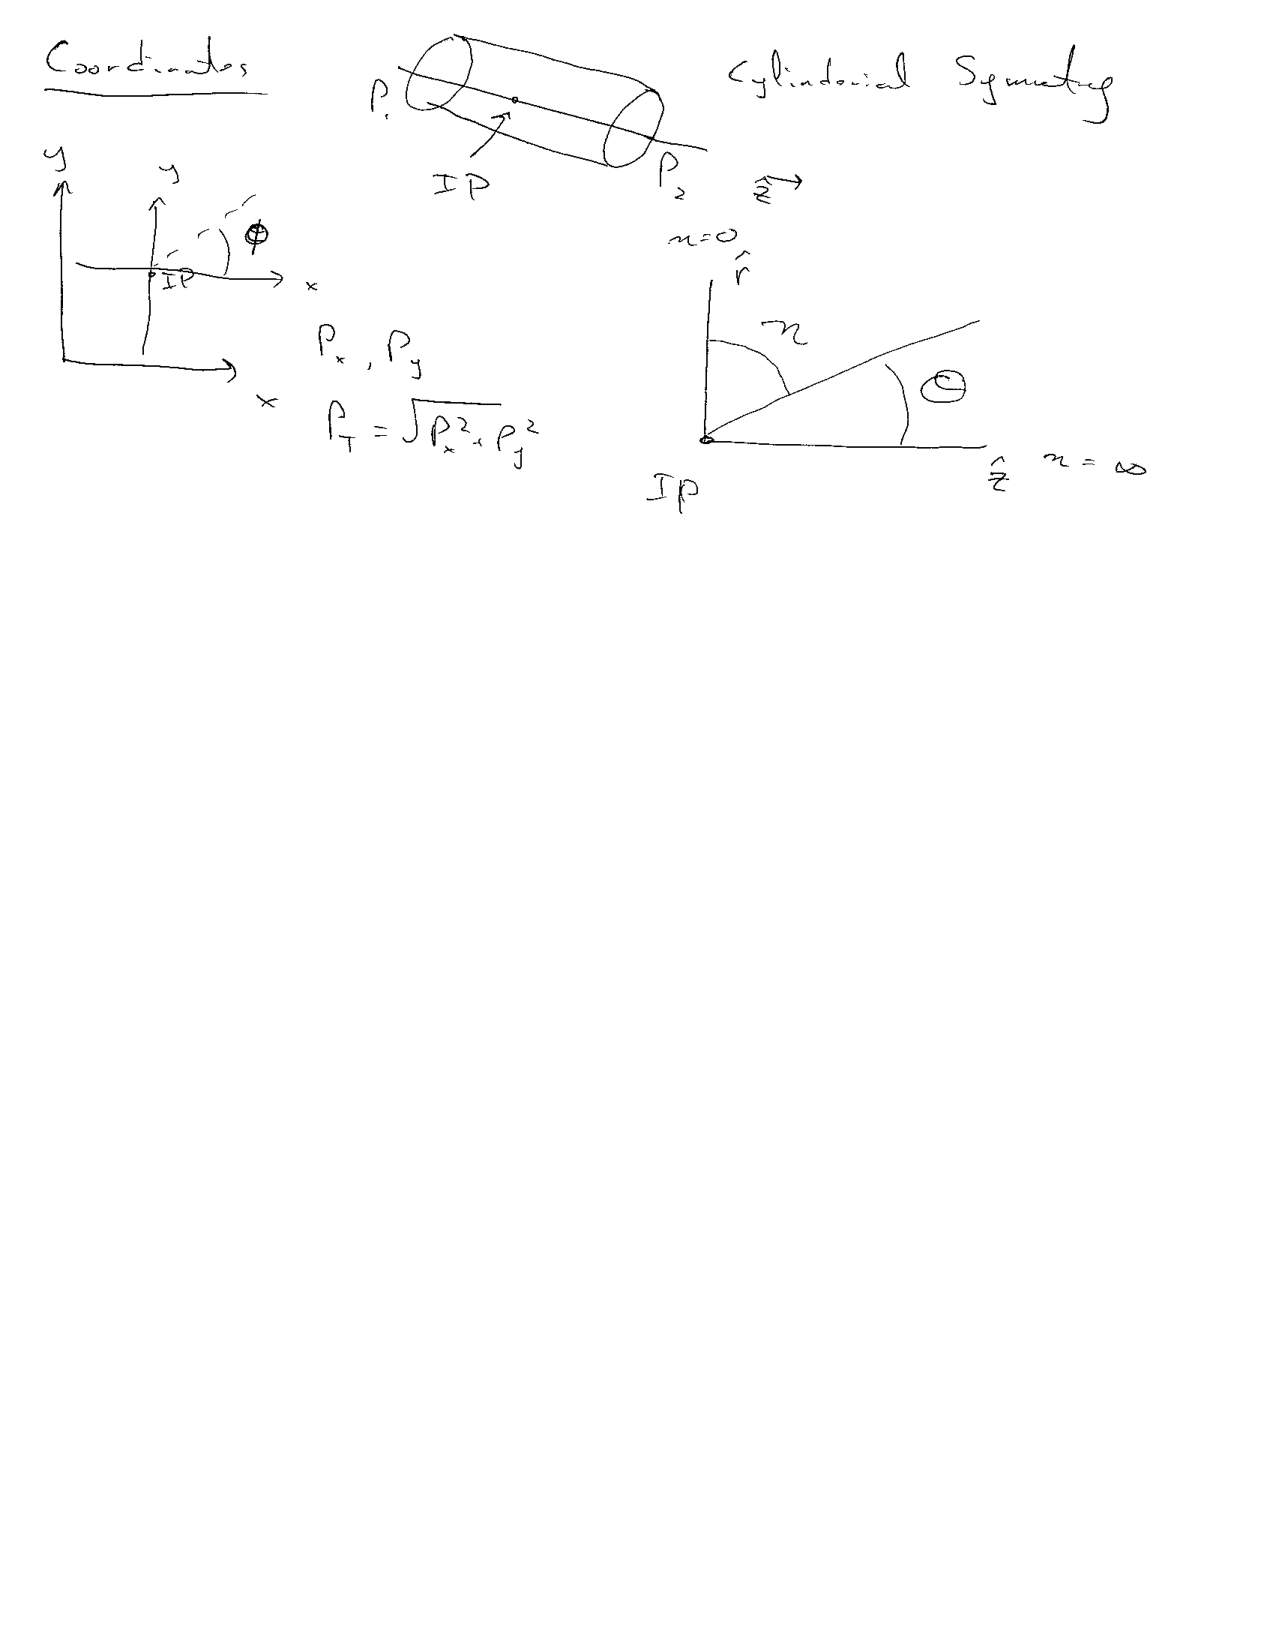
\includegraphics[width=\textwidth]{./Coordinates.pdf}
\ec

``pseudo-rapidity''  (Explore this in HW)
\be
\eta = -\ln \tan \frac{\theta}{2}
\ee

``rapidity''  
\be
y  = \frac{1}{2} \ln \frac{E+p_z}{E-p_z}
\ee

$\eta = y$ for massless particles.


We know $p_T^I$ = 0, we dont know $p_Z^I$, so we are often interested in variables (like $p_T$) that are independent of Boosts along z.


Massless particle:  $p^\mu = p_T(\cosh \eta, \cos \phi, \sin \phi, \sinh \eta)$\\

Massive particle:  $p^\mu = (m_T \cosh y, p_T \cos \phi, p_T sin \phi, m_T \sinh y)$\\
where $m_T = \sqrt{p_T^2 + m^2}$ is called the ``transverse mass'', invariant to boosts along z

\lineacross

In order to be detected, a particle must undergo an interaction with detector material.
(Again this is an enormous subject, we will only scratch surface)


Typically talk about particles loose energy to the detectors. 

Three key mechanisms:

{\Large
\bi
\item[-] Ionisation Energy loss 
\item[-] Radiation Energy loss 
\item[-] Nuclear Interactions
\ei
}

-) Ionisation and Radiation energy loss are long range interactions from the EM force

-) Nuclear Interactions are from the strong or weak force, both short range

-) Ionisation Energy Loss is interaction with electrons in atoms.

-) Radiation Energy Loss and Nuclear Interactions Energy Loss is interaction with atomic nucleus.


\underline{Two Basic Types of Detectors}

\textbf{\underline{Trackers} }
\bi
\item[-] Sensitive to ionization loss
\item[-] Non destructive $\vec{p}_{in} \sim \vec{p}_{out}$
\item[-] Small fraction of energy deposited indicates particle position
\ei


\textbf{\underline{Calorimeters} }
\bi
\item[-] Extract potential energy from Radiation or Nuclear Interactions 
\item[-] Destructive $p_{out}$ = 0
\item[-] Use ionization loss to measure energy of radiation / nuclear interactions 
\ei


\lineacross

\underline{Ionization}

Fast moving particle that interacts electromagnetically with  an electron in an atom.
Particles kicks out electrons, looses energy.

\bc
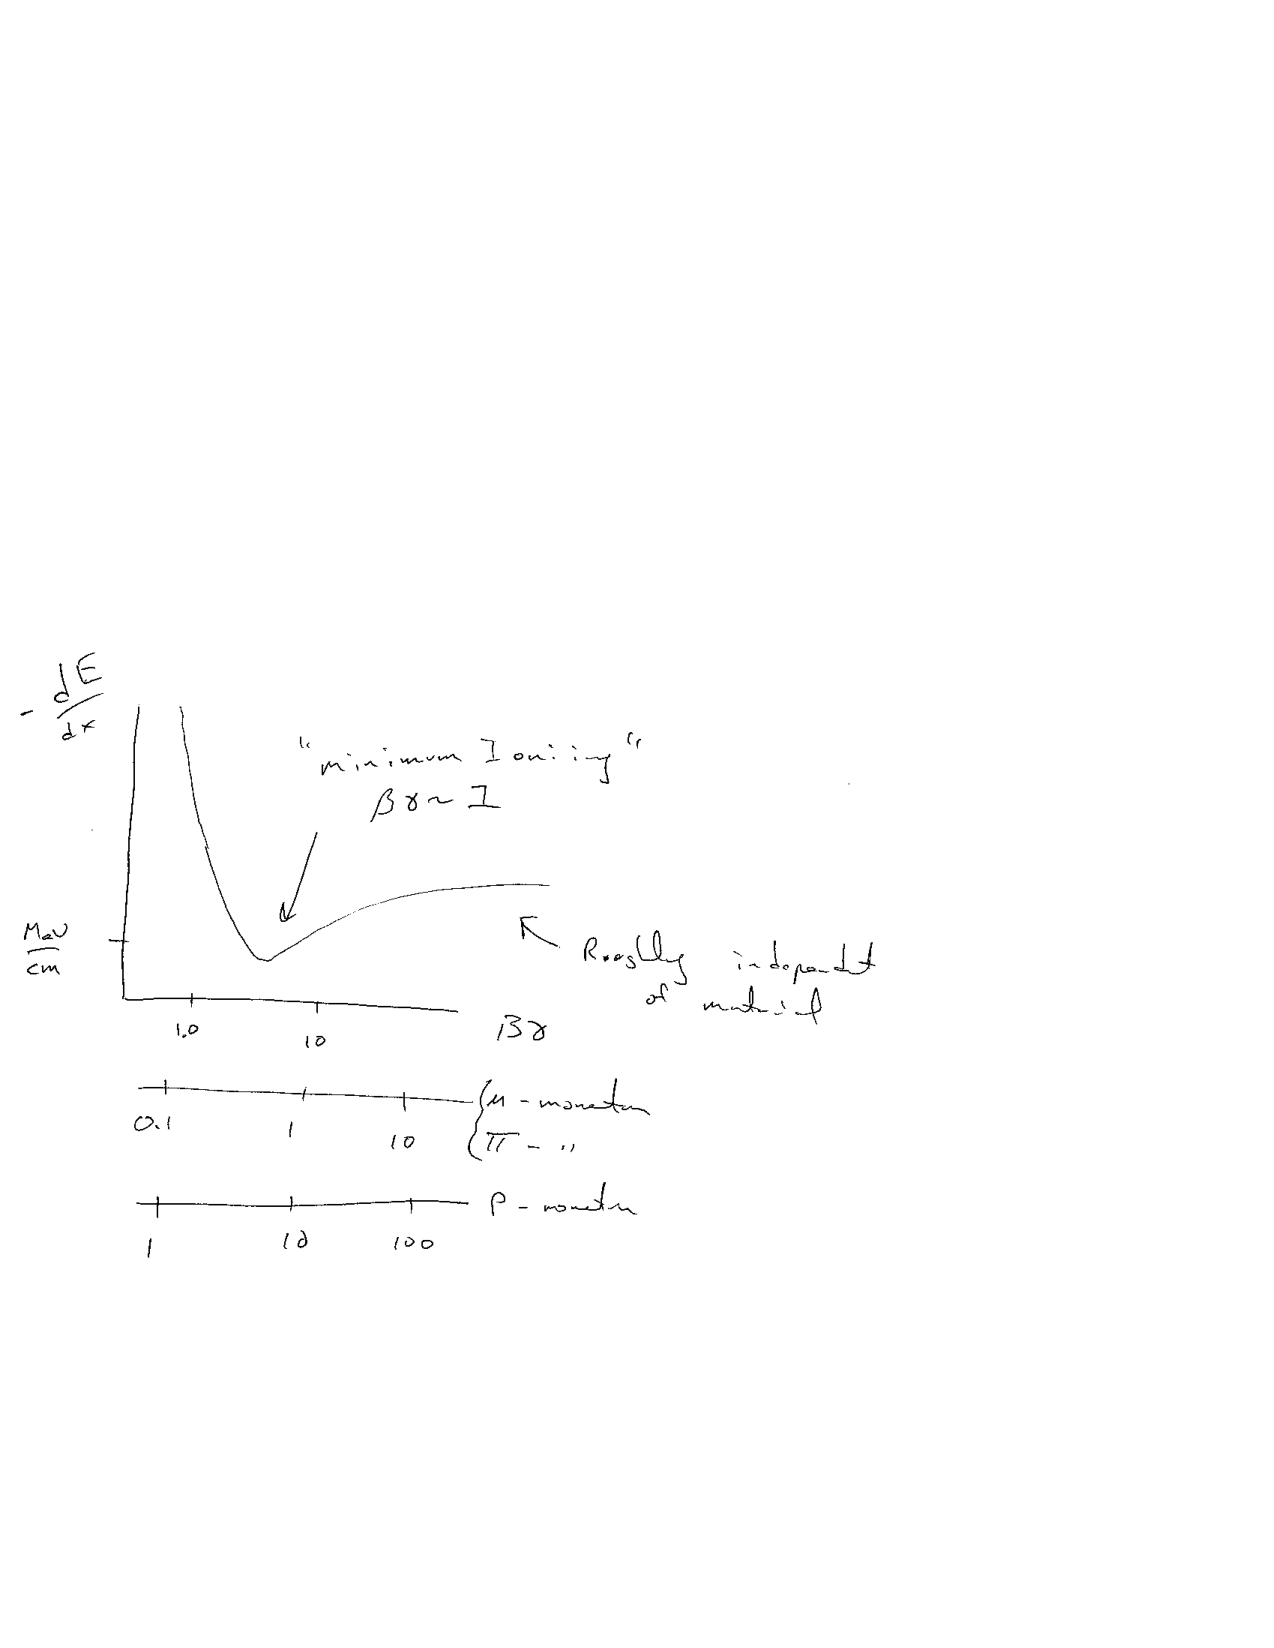
\includegraphics[width=\textwidth]{./DeDx.pdf}
\ec

Ionization dominates as long as particles are not too relativistic: $\beta\gamma \lesssim 1000 $

Above this a new effect takes over ... 

\clearpage

\lineacross

\underline{Radiation Loss}

At very high energy.
\bc
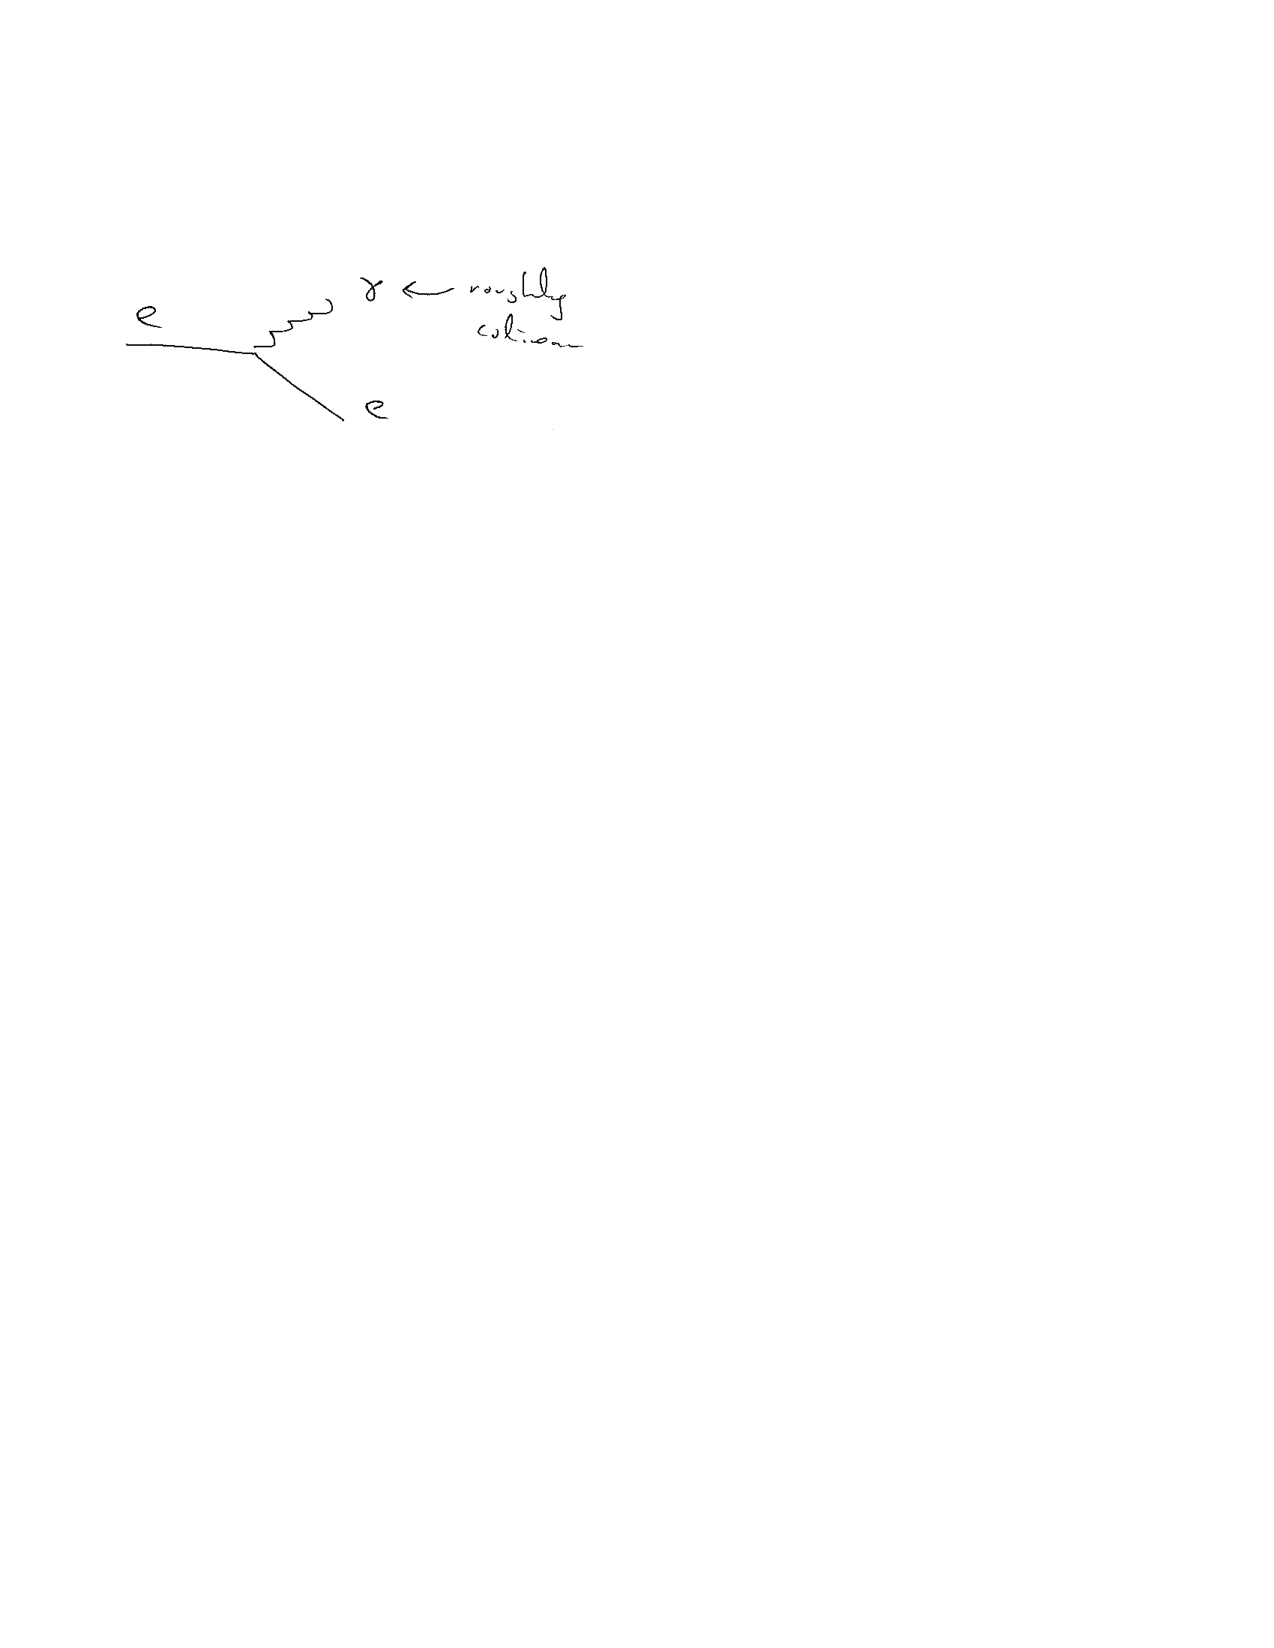
\includegraphics[width=0.6\textwidth]{./Brem.pdf}
\ec
The photon carries a large fraction of the initial energy.

``Bremsstrahlung'' Radiation (German for breaking)


Same effect works for photons
\bc
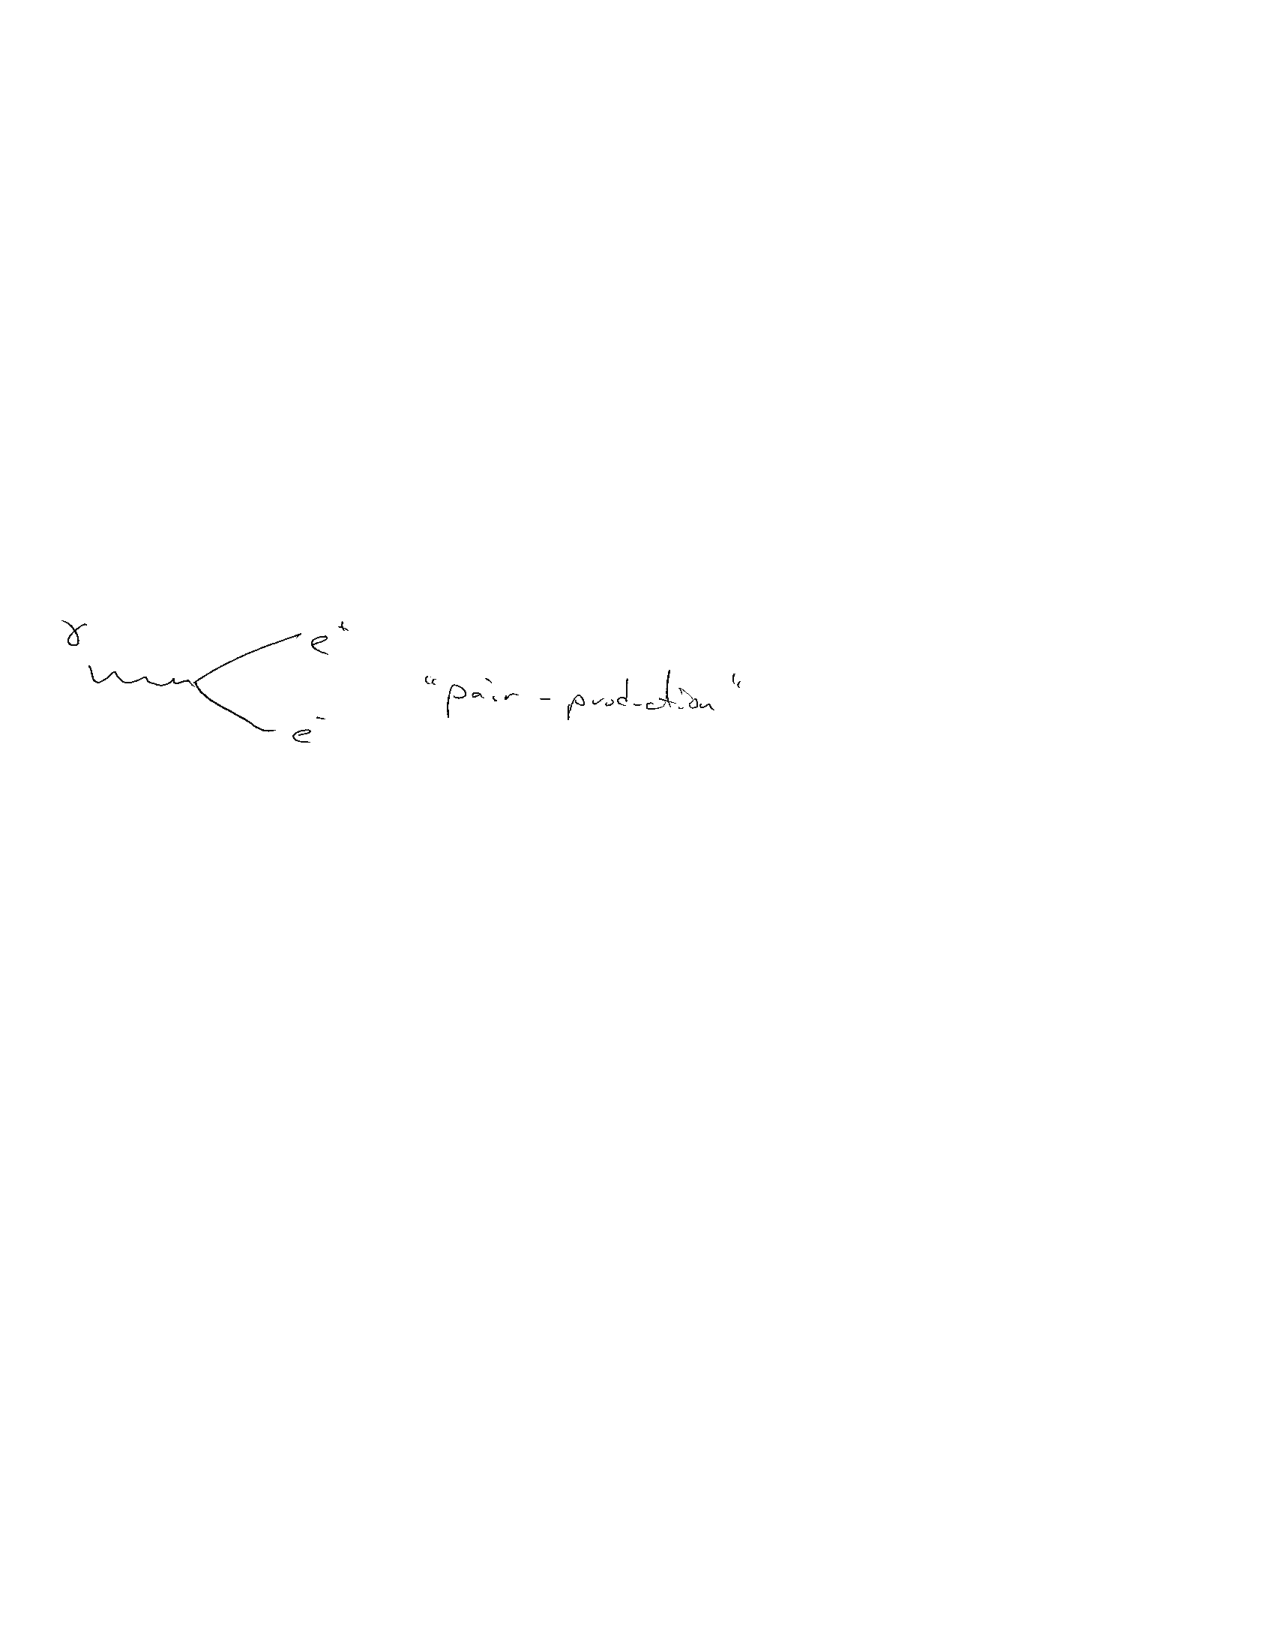
\includegraphics[width=0.8\textwidth]{./PairProduction.pdf}
\ec

Involve interactions with nuclei to conserve four-momentum.


These processes occur infrequently, but are very significant events when they occur.
(Contrasted to Ionization Energy Loss which is $\sim$ continuous and minor)

So here makes sense to talk about the probability for energy loss, not the average along path.

We will skip the details, 

Bottom line:

\be
\frac{dE}{dx} \sim - \frac{E}{x_0}
\ee

$x_0$ - length scale (``radiation length'') distance over which electron looses $e^{-1}$ of its energy. O(cm)


\bc
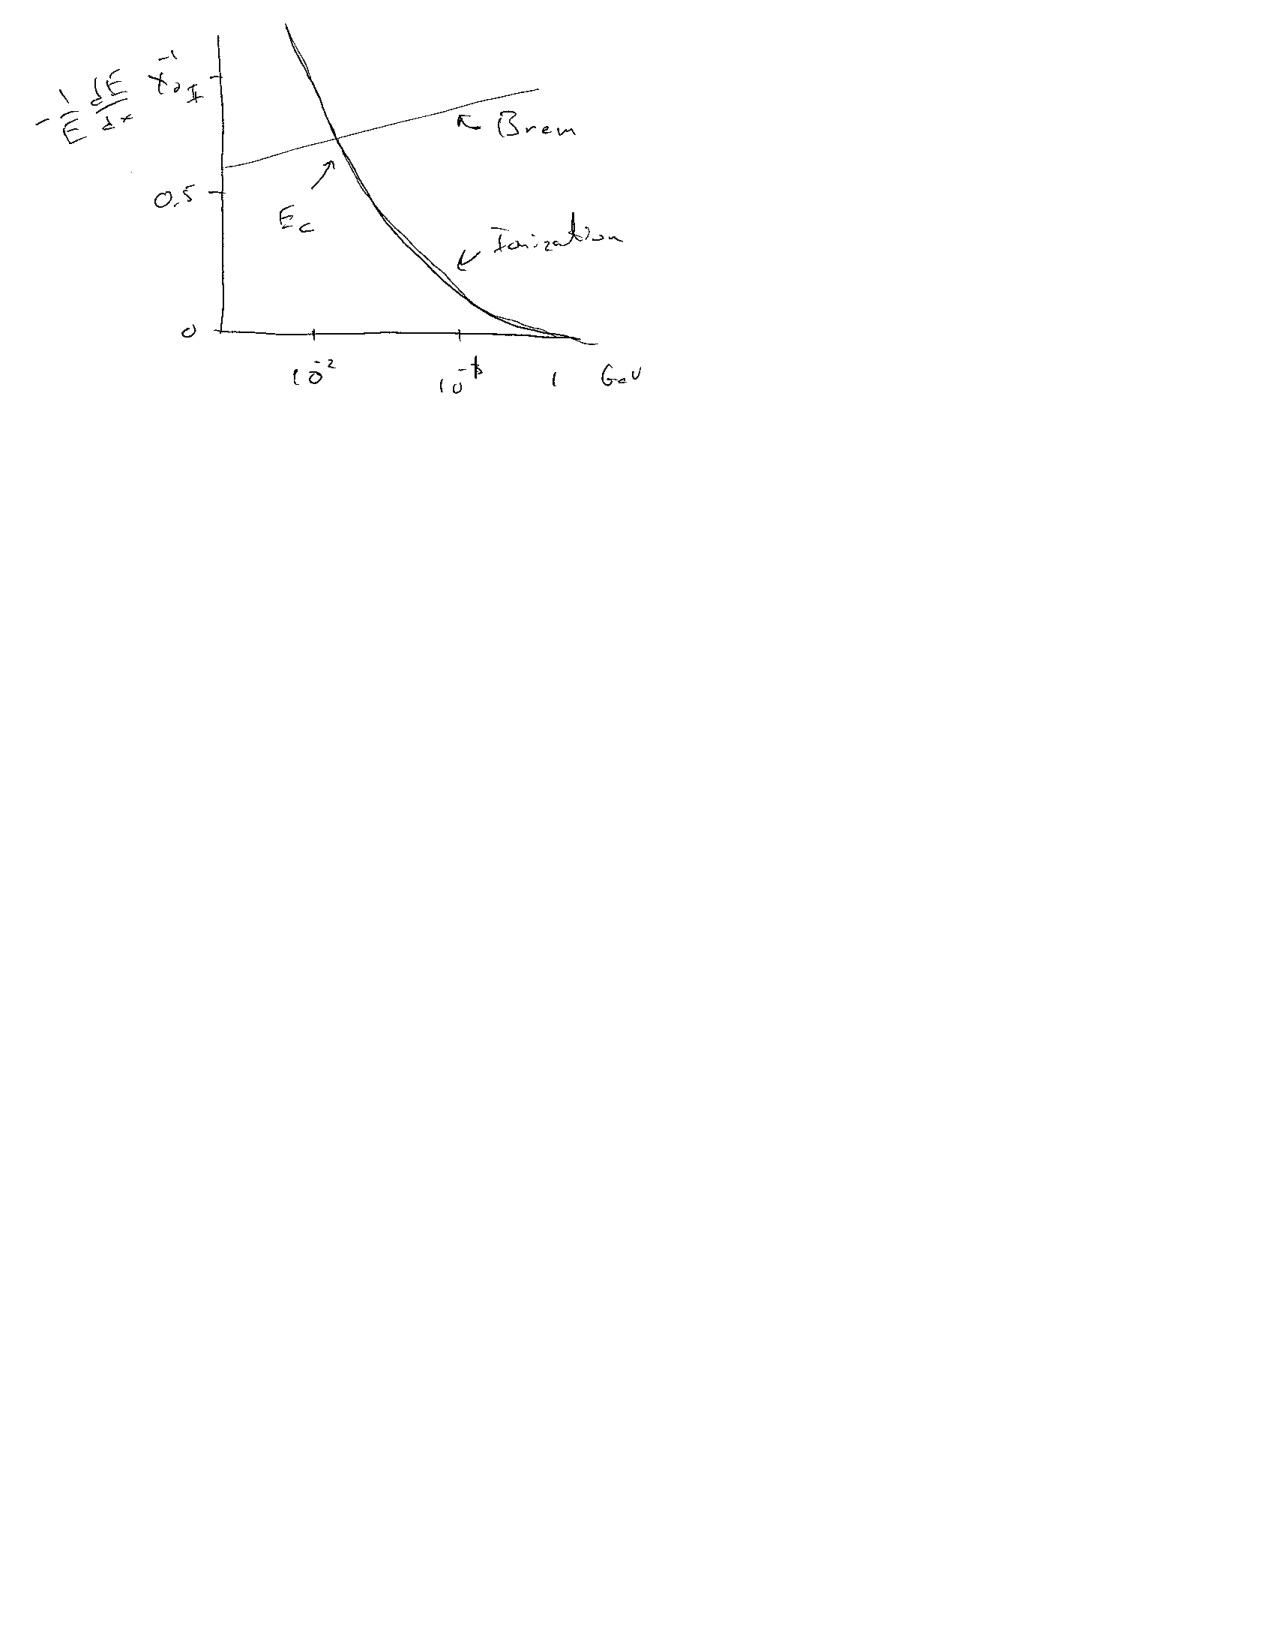
\includegraphics[width=0.8\textwidth]{./DeDxRadiation.pdf}
\ec

Similar story for photons. 

$E_c$ - critical energy O($10^{-2} - 10^{-1}$ GeV)

\begin{minipage}{0.5\textwidth}
\bc
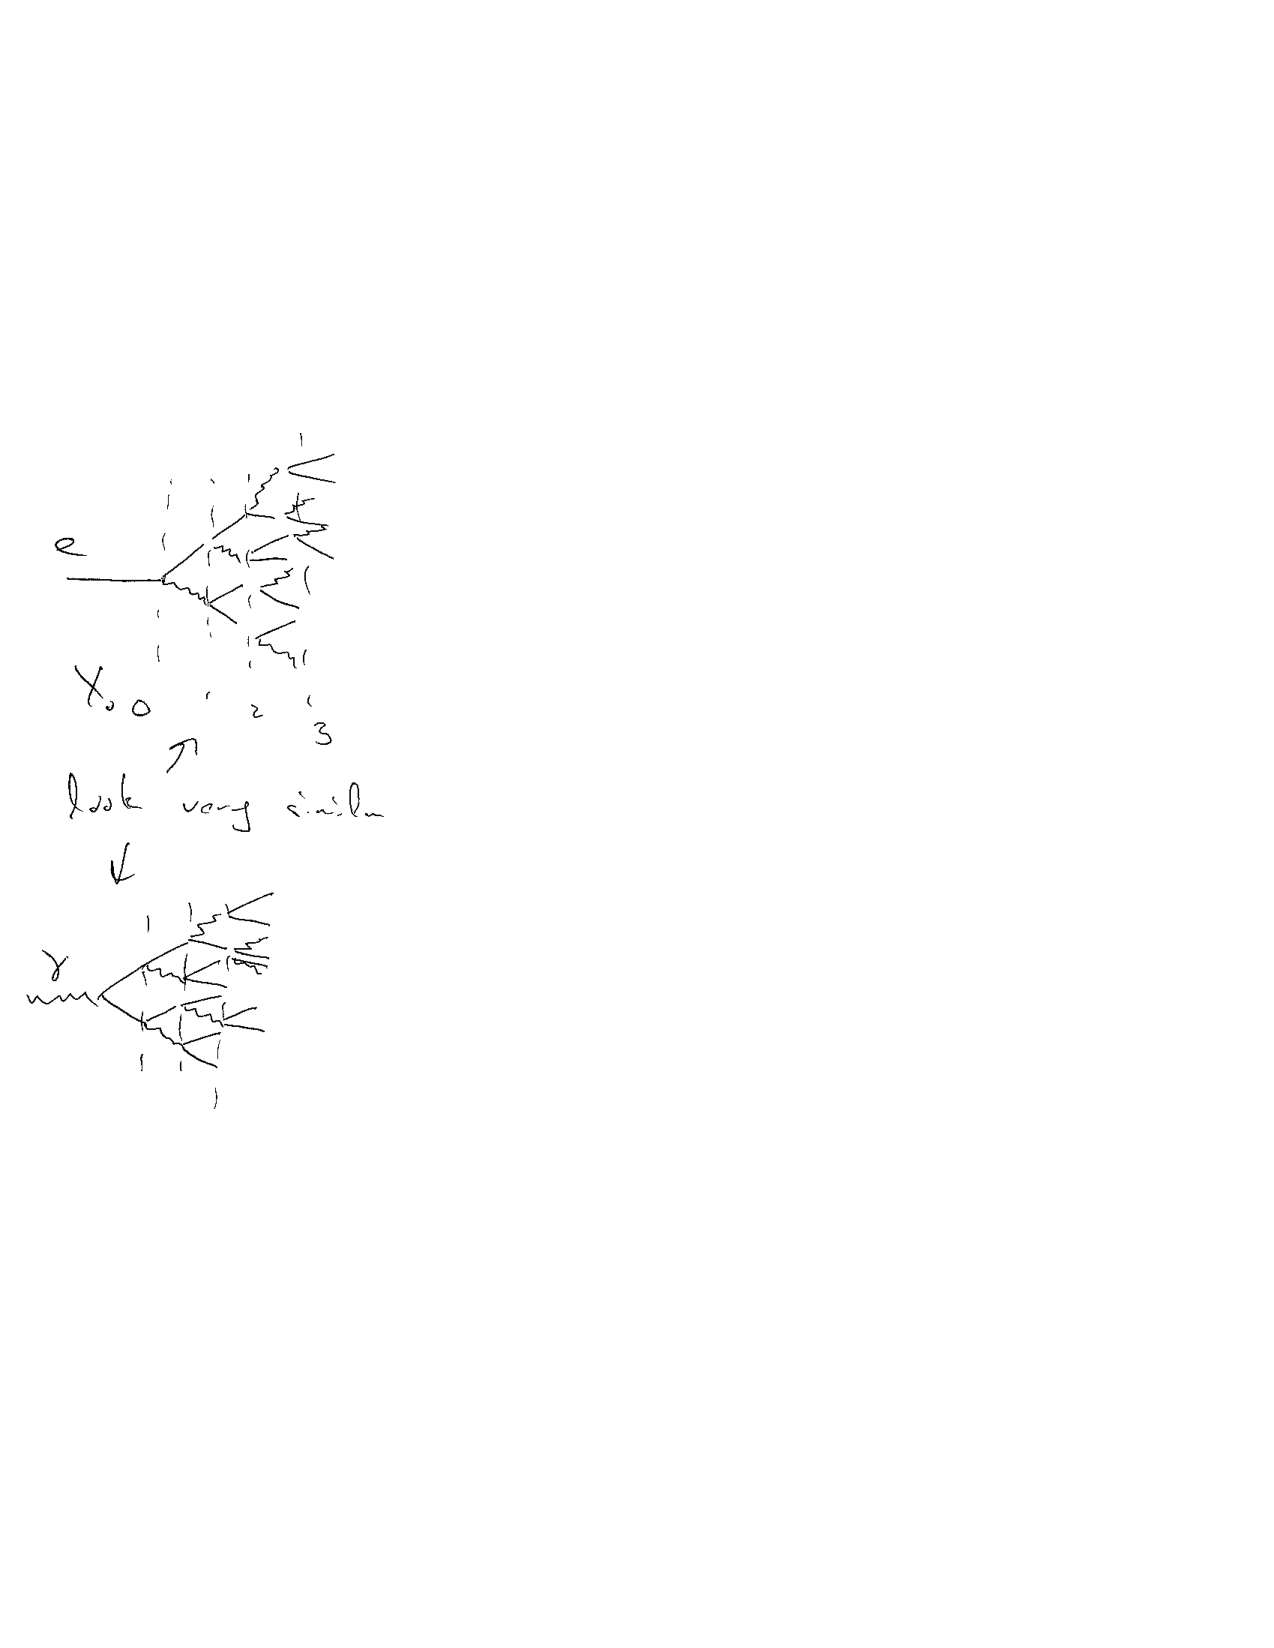
\includegraphics[width=0.8\textwidth]{./EMShower.pdf}
\ec
\end{minipage}\hfill
\begin{minipage}{0.5\textwidth}
\bc
\textbf{``Electromagnetic Shower''}
\ec

-) For each e (or $\gamma$) with $E > E_c$ travels $\sim 1 x_0$ then gives up 1/2 energy to $\gamma$ (or ee).\\

-) e's, $\gamma$'s with energy $< E_c$ get absorbed via ionization\\

If initial energy $E_0 >> E_c$ then after t-radiation lengths there will be $2^t$ particles. 
Approximately equal e's and $\gamma$'s each with energy $E(t) \sim \frac{E_0 }{2^t}$.

\end{minipage} 

Shower will stop growing when 

\be
E(t) \simeq E_c \equiv E(t_{max})
\ee

$t_{max}$ is point in shower with max particles


\be
t_{max} = \frac{\ln \frac{E_0}{E_c}}{\ln 2}
\ee

$\Rightarrow$ shower depth grows as $\ln$

$N_{max}$ given by $E_0/E_c$

}
\end{document}


